%
% File emnlp2018.tex
%
%% Based on the style files for EMNLP 2018, which were
%% Based on the style files for ACL 2018, which were
%% Based on the style files for ACL-2015, with some improvements
%%  taken from the NAACL-2016 style
%% Based on the style files for ACL-2014, which were, in turn,
%% based on ACL-2013, ACL-2012, ACL-2011, ACL-2010, ACL-IJCNLP-2009,
%% EACL-2009, IJCNLP-2008...
%% Based on the style files for EACL 2006 by
%% e.agirre@ehu.es or Sergi.Balari@uab.es
%% and that of ACL 08 by Joakim Nivre and Noah Smith

\documentclass[11pt,a4paper]{article}
\usepackage[hyperref]{emnlp2018}
\usepackage{times}
\usepackage{latexsym}
\usepackage{url}
\usepackage{mathptmx} 
\usepackage{amsmath}


%\aclfinalcopy % Uncomment this line for the final submission

%\def\aclpaperid{***} %  Enter the acl Paper ID here

%\setlength\titlebox{5cm}
% You can expand the titlebox if you need extra space
% to show all the authors. Please do not make the titlebox
% smaller than 5cm (the original size); we will check this
% in the camera-ready version and ask you to change it back.

\usepackage{graphicx}
\graphicspath{{figures/}{pictures/}{figs/}{./}} % where to search for the images
\usepackage{xcolor}  % Coloured text etc.
\usepackage{listings}
\definecolor{codegreen}{rgb}{0,0.6,0}
\definecolor{codegray}{rgb}{0.5,0.5,0.5}
\definecolor{codepurple}{rgb}{0.58,0,0.82}
\definecolor{backcolour}{rgb}{0.95,0.95,0.92}
\lstdefinestyle{mystyle}{
    %backgroundcolor=\color{backcolour},   
    commentstyle=\color{codegreen},
    keywordstyle=\color{magenta},
    numberstyle=\tiny\color{codegray},
    stringstyle=\color{codepurple},
    basicstyle=\scriptsize,
    %basicstyle=\footnotesize,
    breakatwhitespace=false,         
    %breaklines=true,                 
    captionpos=b,                    
    keepspaces=true,                 
    %numbers=left,                    
    %numbersep=1pt,                  
    showspaces=false,                
    showstringspaces=false,
    showtabs=false,                  
    tabsize=1
}

\lstset{style=mystyle}

\newcommand\BibTeX{B{\sc ib}\TeX}
\newcommand\confname{EMNLP 2018}
%\newcommand\conforg{SIGDAT}

\title{Visual Interrogation of Attention-Based Models: \\ Applications in Language Inference and Machine Comprehension}

\author{Shusen Liu \\
  Lawrence Livermore National Laboratory\\
  {\tt liu42@llnl.gov} \\\And
  Tao Li,  Zhimin Li,  Vivek Srikumar, Valerio Pascucci \\
  School of Computing, University of Utah\\
    {\tt {tao.li, zhimin.li, vivek, pacucci}@utah.edu}
} 

\date{}

\begin{document}
\maketitle

\begin{abstract}
Neural networks models have gained unprecedented popularity in natural language processing due to their state-of-the-art performance and the flexible end-to-end training scheme. Despite their advantages, the lack of interpretability hinders the deployment and refinement of the model.
%These models often relying on the attention mechanism, which not only helps improve predicting performance but also provide interpretable representations for users to peak into the opaque models that are usually considered as black boxes.
%
In this work, we present a flexible visualization library for creating customized visual analytic environments, in which the user can investigate and interrogate the relationship among the input, the model internals (i.e., attention), and the output predictions that in turn shed light on the model decision making processing.
 
\end{abstract}


\section{Introduction}


exploration task

Comparsion with AllenNLP


\section{Related Works}
With the increasing demands for model accountability (e.g., what is the evidence for making the decision) and model fairness (e.g., is the prediction affected by the bias in the training data),
the interpretability of the machine learning model held significant implications. As a result, a wealth of researches have be focused on the explanation and interpretation of deep neural network models from both machine learning as well as visualization community.

\noindent\textbf{Model Interpretability.}
Before one can solve the model interpertability challenge, we first need to understand what constitute an explaination or interpretation of a machine learning model.
As discussed in ~\cite{Lipton2016, Doshi-Velez2017}, the concept of interprebale is inherently subjective, since the recipients of the explaination are always human.
% And the discussion of interpretability quickly become philosophical.
However, despite the underspecification nature of the problem, we can still refine the concept and provide certain guideline~\cite{Doshi-Velez2017}.

One of the most studied aread in model interpretability is the explanation of a given prediction.
Many works have been dedicated to providing intuitive explanations for a given prediction, several~\cite{RibeiroSinghGuestrin2016, KrausePererNg2016} of which approach the problem from a model agnostic approach that made them applicable to different applications (i.e., by fitting a simplier linear model near the prediction of interests).
%
Despite being invaluable for the providing human understandable explanation, the lack of the ability to access and explore the internal states of the model, which is vitally important to make sense of why a model fail, limits their ability for more in depth exploration and evaluation of the model.
% (Limitation of the state-of-the arts)
% Model independent explanations is useful to gain intuition, but they lack the ability to link the external observation with inner states/mechanism of the model.

\noindent\textbf{Visual Interpration of Neural Networks.}
The effectiveness in the exploration of complex relationships, visualization have long been adopted for interpreting neural network models (e.g., the early works such as~\cite{TzengMa2005})
Recently, many visualization works has dedicated to the neural network model interpretability challenges.
% The classification~\cite{KrausePererNg2016}
In the work~\cite{BilalJourablooYe2018} by Bilal et al., the authors analyzing classification errors in convolutional neural networks and answer the question on whether class hierarchy is learn in the network.
Liu et al.~\cite{LiuShiCao2018} explore the possiblility of understanding the training process of deep generative models.
The ActiVis~\cite{KahngAndrewsKalro2018} focus on large scale network in real world setting.
The DeepEyes~\cite{Pezzotti2018} focuses on the analyzing the training procss, so they can provide design guideline to the deep neutral network architect.

% \begin{itemize}
%     \item ActiVis: Visual Exploration of Industry-Scale Deep Neural Network Models
%     \item Analyzing the Training Processes of Deep Generative Models
%     \item Visual Diagnosis of Tree Boosting Methods
%     \item TreePOD: Sensitivity-Aware Selection of Pareto-Optimal Decision Trees
%     \item LSTMVis: A Tool for Visual Analysis of Hidden State Dynamics in Recurrent Neural Networks
%     \item Do Convolutional Neural Networks learn Class Hierarchy?
%     \item DeepEyes: Progressive Visual Analytics for Designing Deep Neural Networks
% \end{itemize}

\noindent\textbf{Neural Linguistic Model Visualization.}
Compare to the multitude of researchs for making sense of convolutional neural networks, relatively less works has been dedicated to neural linguistic models.
%
However, the previous works~\cite{KarpathyJohnson2015, LiChenHovy2015, StrobeltGehrmannPfister2018, LiuBremerJayaraman2018} not only demonstrated the benefit of visualization in understanding NLP models, but also revealed enoumous possibility for future applications.
% There is many unresolve challenge and the
The early work on charactor level recurrent network~\cite{KarpathyJohnson2015} demonstrates effectness of the hidden state in capturing the unique pattern in training text. The compositionality exibited in neural linguistic model (i.e., build sentence from meaing of words and phrases) are examined in the work by Li et al. ~\cite{LiChenHovy2015}, by utilizing methods inspired by similar work in computer vision.
The LSTMvis~\cite{StrobeltGehrmannPfister2018} work utilized a line plot style visual encoding to visualize the time varying hidden states of recurent neutural network. The word embedding visualization work~\cite{LiuBremerJayaraman2018} illustrate how semantic relationship can be recovered by linear projections in the high-dimensional word embedding space produced by word2vec~\cite{MikolovSutskeverChen2013} or glove~\cite{PenningtonSocherManning2014}.

\section{System}

%\begin{figure*}[t]
%\centering
%\vspace{-2mm}
% 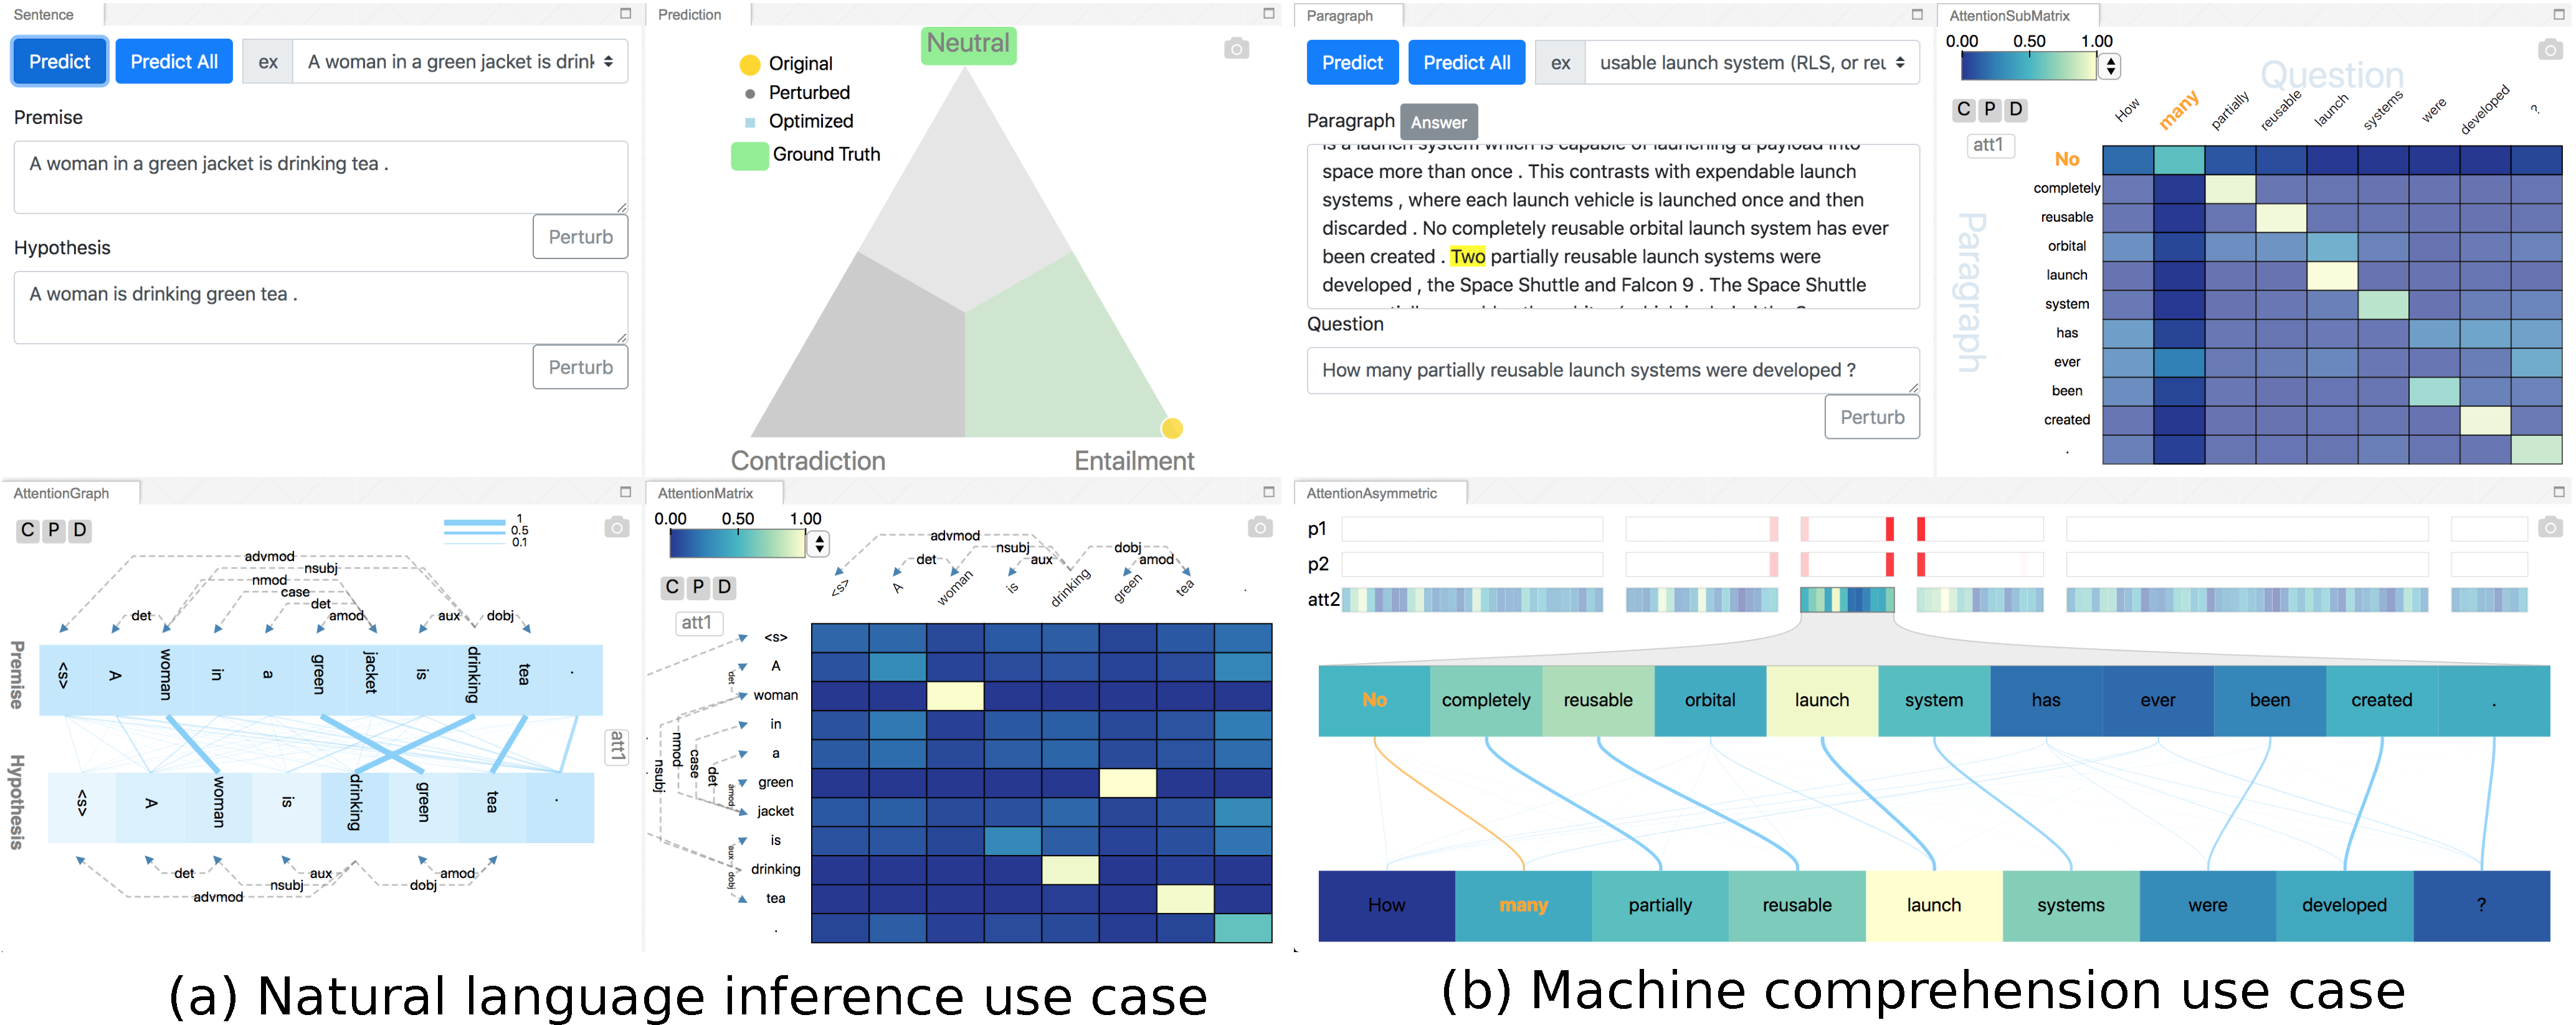
\includegraphics[width=1.0\linewidth]{NLI_MC_interface}
%  \vspace{-6mm}
% \caption{
%Illustration of different configurations for the natural language inference and machine comprehension tasks.
%}
%\label{fig:pipelineUpdate}
%\end{figure*}
\begin{figure*}[t]
\centering
 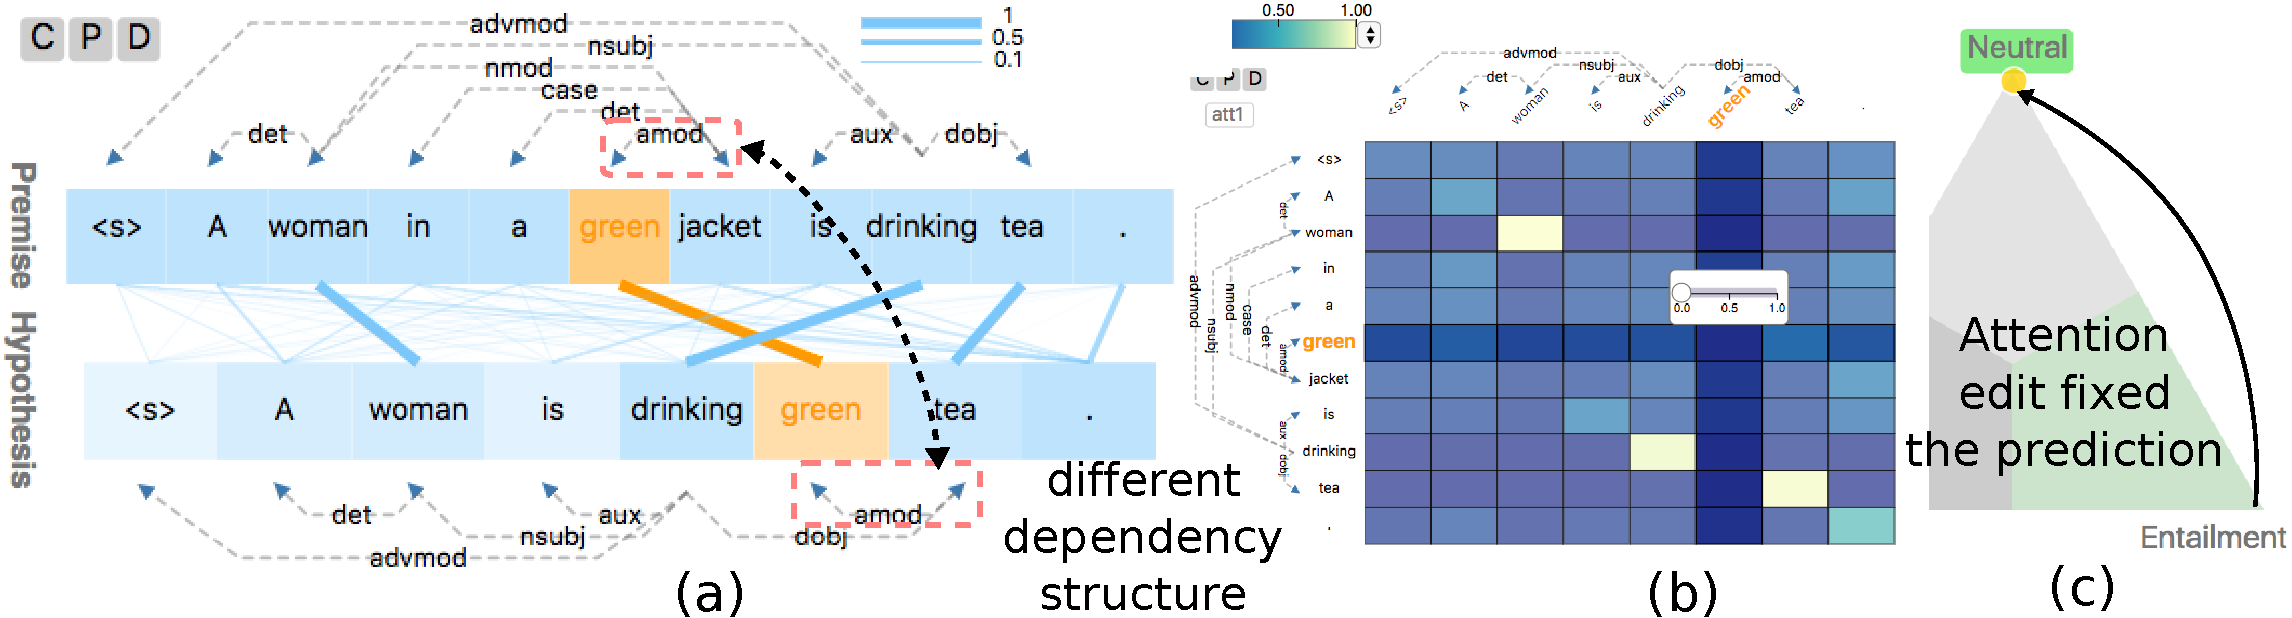
\includegraphics[width=1.0\linewidth]{NLIexample}
  \vspace{-6mm}
 \caption{
An illustration of the attention editing process.
The dependency structure is shown in (a), where the two ``greens'' decorate different nouns.
By removing the ``wrong'' alignment in (b), the original prediction \emph{entailment} is corrected to \emph{neutral} in (c).
}
\label{fig:NLIexample}
\end{figure*}

\section{Applications}
We demonstrate the proposed visualization system on the decomposable attention network~\cite{parikh2016emnlp}
for the NLI task and the BIDAF model~\cite{Seo2016} for the MC task.

\subsection{Natural Language Inference}
\label{sec:NLIexample}
The NLI task predicts the entailment relationship between a premise sentence (P) and a hypothesis sentence (H).
The attention matrix captures the alignment of words between these two sentences.
Here we give an example of how a wrong prediction can be corrected by editing attention values.  

%The model produces two attention matrices, representing alignment from premise to hypothesis, and from hypothesis to premise.
%as either \emph{entailment}, \emph{contradiction}, or \emph{neutral}.
%The model can be formalized as the following:
%%\begin{align}
%	$P^\prime, H^\prime = f(P), f(H)$,
%	$\overleftarrow{A} = P^\prime \cdot H^\prime$,
%	$\overrightarrow{A} = H^\prime \cdot P^\prime$,
%	$y = g(P, H, P^\prime, H^\prime, \overleftarrow{A}, \overrightarrow{A})$,
%%\end{align}
%where $P$ and $H$ are input embedding matrices for the premise and the hypothesis, $\overleftarrow{A}$
%and $\overrightarrow{A}$ are attentions, and $y$ is the predicted probabilities for candidate classes.
%Our system visualized the bidirectional attentions and their interaction with output distribution over labels.

As illustrated in Fig.~\ref{fig:NLIexample}(a), the input sentence pair (P:``A woman in a green jacket is drinking tea.'' H:``A woman is drinking green tea.'') is predicted to be \emph{entailment}, which is incorrect.
By examining the attention, we can see the word \emph{green} in ``\emph{green} jacket" is aligned to the \emph{green} in ``\emph{green} tea." However, these two \emph{greens} modify different nouns, which potentially leads to the wrong prediction. The grammatical structure is visually shown in the form of the dependency tree.
%i.e., \emph{green} in \textbf{P} is attached to ``jacket''.
However, the model does not have access to the syntactic information and mistakenly assumes the two \emph{greens} modify the same thing.
% (thus predict \emph{entailment}). 
%
To correct the mistake, we can edit the attention value and remove the align between these two ``greens" (see (c)(b)).
As expected, the prediction label is corrected (\emph{neutral}).

\begin{figure*}[t]
\centering
 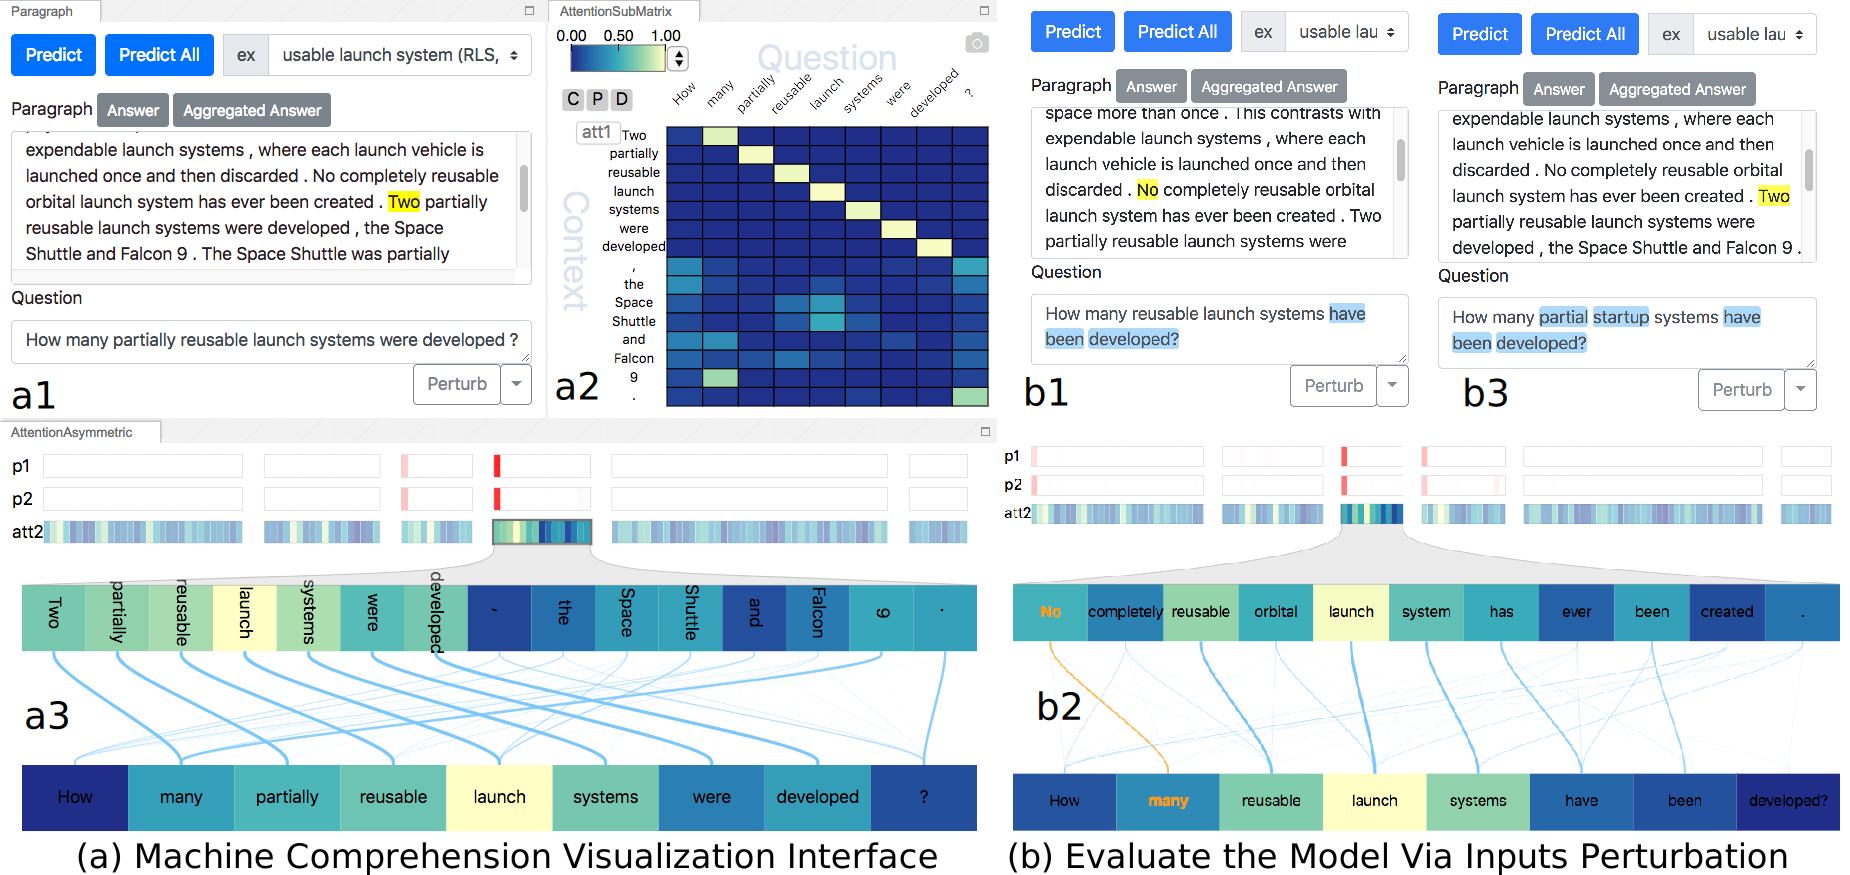
\includegraphics[width=1.0\linewidth]{MC_interface}
  \vspace{-6mm}
 \caption{
In the machine comprehension visualization interface (a), the $p1$, $p2$ colored bar (in $a3$) illustrates the predicted start and end index of the answer in the context (the deeper the red, the higher the probability). The most likely answer is shown in ($a1$). The global attention and local attention are visualized by ($a2$, $a3$).
%
We can evaluate the robustness of the prediction by perturbing the question sentence ($b1$, $b3$). As illustrated in ($b1$, $b2$), by removing the word ``partial'', the model still finds the correct answer (albeit different, as the sentence perturbation changes the exact meaning of the question). 
}
\vspace{-2mm}
\label{fig:MCexample}
\end{figure*}

\subsection{Machine Comprehension}
\label{sec:MCexample}
In the machine comprehension task, the goal is to select a span of text as the answer
to a question sentence.
%two sequences of texts are given: context and question.
%The goal is to select a span of text from the context that answers the question. 
%We provide a simple model formulation and refer the reader to the paper for details.
%%\begin{align}
%	$C^\prime, Q^\prime = BiLSTM(C), BiLSTM(Q)$,
%	$\overleftarrow{A} = u(C^\prime, Q^\prime)$,
%	$\overrightarrow{A} = v(C^\prime, Q^\prime)$,
%	$s = m(C^\prime, Q^\prime, \overleftarrow{A}, \overrightarrow{A})$,
%	$e = n(s, C^\prime, Q^\prime, \overleftarrow{A}, \overrightarrow{A})$,
%%\end{align}
%where $C$ and $Q$ are embedding matrices for the context and the question,
%$\overleftarrow{A}$ and $\overrightarrow{A}$ are bidirectional attention flows,
%$s$ and $e$ are probabilities for starting and ending indices of the answer span.
%Our system reveals the internal states of $\overleftarrow{A}$, $\overrightarrow{A}$,
%$s$ and $e$.
The attention information is encoded as a bidirectional alignment (i.e., from context to question and vice versa). 
%The key difference is how the question to context alignment is computed (see \cite{Seo2016} for more details).
Here, we refer the context to question attention as \emph{att1} and the question to context attention as \emph{att2} (which is a vector instead of a matrix according to \citet{Seo2016}). In this demo, we apply a min max normalization for \emph{att2} after the softmax layer to better distinguish different attention values.

As illustrated in Figure~\ref{fig:MCexample}, we represent \emph{att2} as colored bars with a \emph{yellow-green-blue} colormap. Each rectangular bar corresponds to one sentence. The user can focus on individual sentences by clicking on the rectangular bar (see Figure~\ref{fig:MCexample}).
%The proposed visualization help reveal the potential alignment issues in the machine comprehension model.
The $p1$, $p2$ colored bars (\emph{white-red} colormap) illustrate the predicted probabilities of the start and the end index for the answer (the deeper the higher). %The span of text defined by the beginning and end index with the highest probability is the answer.
%
%In Figure~\ref{fig:MCexample} ($a3$), there are two spans of text that correspond to higher probabilities. 
In Figure~\ref{fig:MCexample}(a3), the sentence containing the answer exhibits good alignment with the question (e.g., ``Two'' with ``many'').
%In (a3), we examine the sentence that contains the answer, which exhibits excellent alignment with the question (e.g., ``Two'' is aligned with ``many''). 
%The spans of text with high probability are ``Two'' and ``No'' (highlight in orange), both align well with the word ``many''.
Interestingly, the number ``9" (in ``Falcon 9") is also aligned with ``many", which may lead to problems.

The user can explore the robustness of the model by examining how the prediction varies when the question is perturbed.
%
As illustrated in ($b1$, and $b2$), the perturbation removes the word ``partial" in the original sentence, which leads the model to produce a different yet correct answer (``No"). Referring to ($a1$), we can see the word ``No" exhibits the second highest probability for the original question.
%
The user can also manually edit the text. As shown in ($b3$), the model still produces the correct answer when changing the question from ``how many" to ``which".
%One possible explanation is that the word ``Two'' has a much higher \emph{att2} attention value compared to ``9'', which may contribute to the current outcome.

%%% Local Variables:
%%% mode: latex
%%% TeX-master: "NLPVis-demo-paper"
%%% End:


\bibliographystyle{acl_natbib_nourl}
\bibliography{NLPvis.bib}

\end{document}
